\chapter{Verification and Evaluation}
\label{ch:evaluation}

This chapter presents the verification methodology, the detailed results of functional
testing at unit and system level, performance benchmarks measured in simulation, and
FPGA synthesis results that characterise the timing and area of the design. It also
documents the open issues remaining after the current implementation.

% ===========================================================================
\section{Verification Methodology}
\label{sec:verif_method}

\subsection{V-Model Approach}

The verification strategy follows a V-model structure in which each level of abstraction
on the design side has a corresponding verification artefact on the test side. Three
levels of verification were employed:

\begin{enumerate}
  \item \textbf{Unit level}: Each functional sub-unit of the VPU (\texttt{vproc\_adder},
        \texttt{vproc\_mul}, \texttt{vproc\_shifter}, \texttt{vproc\_compare},
        \texttt{vproc\_reduction}, \texttt{vproc\_vec\_lsu}) is exercised in isolation
        through directed test vectors that target arithmetic boundaries, sign-extension
        paths, and handshaking edge cases.
  \item \textbf{Integration level}: The complete \texttt{vproc\_system\_wrapper} (VPU
        without the scalar core) is exercised by the 172-test regression
        (\texttt{tb\_vproc\_all\_instr.sv}), which covers all supported opcode categories
        and representative combinations of operand types (VV, VX, VI), LMUL settings,
        and widening.
  \item \textbf{System level}: The full \texttt{riscv\_vpu\_top} (scalar core + VPU) is
        exercised by the \texttt{tb\_lena\_gray.sv} testbench, which pre-loads the
        128$\times$128 Lena RGB image into DMEM and verifies pixel-level accuracy of the
        BT.601 grayscale output against a Python-computed reference.
\end{enumerate}

\subsection{Simulation Environment}

All simulations use ModelSim (Siemens EDA) in 64-bit mode. SystemVerilog testbenches
are compiled with \texttt{vlog -sv}, and simulation is launched with
\texttt{vsim -voptargs=+acc} to enable full visibility of all internal signals and
hierarchical hierarchy access from the testbench tasks. The \texttt{+acc} flag is
necessary for the VRF read/write helper tasks in \texttt{tb\_vproc\_all\_instr.sv},
which access internal arrays of \texttt{vproc\_vregfile} directly by hierarchical path.

Each test class has a dedicated \texttt{.do} script in the project root:
\texttt{vproc\_all\_instr.do} for the VPU instruction regression,
\texttt{run\_top\_sim.do} for the integrated scalar + VPU smoke test, and
\texttt{run\_lena\_sim.do} for the full 128$\times$128 image benchmark. All scripts
compile from source and load the required hex firmware into IMEM before starting.

\subsection{Regression Gate Policy}

A design change is considered complete only when the full 172-test regression
(\texttt{vproc\_all\_instr.do}) reports \texttt{PASS} for every test case. This
regression gate was enforced for every modification to any \gls{rtl} module in the
\texttt{/rtl/} hierarchy, including the four-operand-type extension for the compare
unit, the LMUL accumulation loop, and the serial reduction redesign.

% ===========================================================================
\section{Unit-Level Verification}
\label{sec:unit_verif}

\subsection{Adder Unit (\texttt{vproc\_adder})}

The adder unit handles \texttt{vadd}, \texttt{vsub}, and \texttt{vrsub}. Unit tests
exercise the following cases:

\begin{itemize}
  \item \textbf{Positive addition:} $100 + 200 = 300$ at all three \gls{sew} widths
        (8, 16, 32 bits).
  \item \textbf{Unsigned wraparound:} at SEW=8, $255 + 1 = 0$ (no carry into the next
        element).
  \item \textbf{Subtraction with borrow:} $10 - 50 = -40$, verified to produce the
        correct two's complement result at SEW=32.
  \item \textbf{VRSUB operand swap:} \texttt{vrsub.vx} computes $\mathrm{rs1} -
        \mathrm{vs2}[i]$; the test verifies that $10 - [1,2,3,4] = [9,8,7,6]$ across
        all four lanes, confirming that the operand-swap mux is correctly gated by the
        \texttt{is\_reverse\_sub} control bit.
  \item \textbf{Signed boundary:} SEW=32, $0x7\mathrm{FFFFFFF} + 1 = 0x80000000$
        (maximum positive to minimum negative transition).
\end{itemize}

\subsection{Multiplier Unit (\texttt{vproc\_mul})}

The multiplier handles the full VMULH family. Corner cases tested include:

\begin{itemize}
  \item \textbf{Low-half correctness:} $3 \times 4 = 12$ at SEW=32, verifying the
        low-half write path used by \texttt{vmul.vv}.
  \item \textbf{High-half signed (\texttt{vmulh}):} $0x10000 \times 0x10000 = 2^{32}$;
        the high 32 bits equal 1. Also tested at SEW=32: $0x40000000 \times 4 = 2^{32}$,
        high 32 bits = 1.
  \item \textbf{High-half unsigned (\texttt{vmulhu}):} $0x80000000 \times 0x80000000 =
        2^{62}$; high 32 bits = \texttt{0x40000000}.
  \item \textbf{Mixed-sign (\texttt{vmulhsu}):} vs2 treated as signed ($-2^{31} =
        0x80000000$), vs1 treated as unsigned ($2$); product $= -2^{32}$; high 32 bits
        $= 0\mathrm{xFFFFFFFF}$.
  \item \textbf{Widening multiply (\texttt{vmulw}):} $3 \times 4 = 12$ at SEW=32,
        result written as 64 bits across two consecutive destination registers (lo=12,
        hi=0).
\end{itemize}

\subsection{Reduction Unit (\texttt{vproc\_reduction})}

The reduction unit receives the serial element stream and accumulates into a single
scalar result. Tests verify:

\begin{itemize}
  \item \textbf{VREDSUM:} $\{5, 12, 3, 8\}$, initial accumulator = 0, expected sum = 28.
  \item \textbf{VREDMAX signed:} same input, expected maximum = 12.
  \item \textbf{VREDMIN signed:} $\{-5, -12, -3, -8\}$, expected minimum = $-12$
        ($0\mathrm{xFFFFFFF4}$), verifying that the signed comparison correctly handles
        negative values.
  \item \textbf{VREDMAXU unsigned:} $\{0\mathrm{xFFFFFFF0}, 1, 2, 3\}$, expected
        maximum = $0\mathrm{xFFFFFFF0}$ (the large unsigned value), verifying that the
        unsigned-mode comparator is selected when \texttt{minmax\_is\_unsign} is set.
  \item \textbf{VREDMINU unsigned:} $\{0, 5, 3, 2\}$, expected minimum = 0.
  \item \textbf{Multi-chunk, LMUL=2:} eight-element reduction across two register groups,
        verifying that the LMUL loop correctly feeds all eight elements to the accumulator
        before asserting the done signal.
  \item \textbf{Busy handshake:} confirms that \texttt{reduction\_busy} is asserted
        for exactly as many cycles as the element count and that the result is written
        to vd[lane0] immediately after the final element is processed.
\end{itemize}

\subsection{Vector LSU (\texttt{vproc\_vec\_lsu})}

The vector load/store unit connects the VPU to DMEM. Tests verify:

\begin{itemize}
  \item \textbf{Unit-stride load at all SEW widths:} \texttt{vle8.v}, \texttt{vle16.v},
        and \texttt{vle32.v} each produce correct data from contiguous DMEM addresses.
  \item \textbf{Store byte-enables:} \texttt{vse8.v} asserts \texttt{vlsu\_mem\_be=4'b0001}
        for each byte-lane transaction; \texttt{vse16.v} asserts \texttt{4'b0011};
        \texttt{vse32.v} asserts \texttt{4'b1111}. The testbench verifies the
        \texttt{mem\_be} signal directly.
  \item \textbf{Masked store:} with \texttt{vm=0} and \texttt{v0} mask = \texttt{4'b1010},
        only elements 1 and 3 generate memory write transactions; elements 0 and 2
        produce no bus request.
  \item \textbf{Address generation:} for a base address of \texttt{0x100} at SEW=32,
        the \gls{vlsu} generates addresses \texttt{0x100}, \texttt{0x104}, \texttt{0x108},
        \texttt{0x10C} for elements 0--3, confirming 4-byte element stride.
\end{itemize}

% ===========================================================================
\section{Instruction Regression (tb\_vproc\_all\_instr)}
\label{sec:regression}

\subsection{Test Structure}

The \texttt{tb\_vproc\_all\_instr.sv} testbench exercises the
\texttt{vproc\_system\_wrapper} directly, bypassing the scalar pipeline. Test vectors
are applied by writing instruction bits and scalar register values directly to the
wrapper's input ports. The VRF is preloaded using a hierarchical write task that
writes all four lane banks simultaneously, and the result is read back through an
identical hierarchical read task after the FSM returns to \texttt{ST\_IDLE}.

The test body is organised into thirteen numbered sections, each covering a distinct
opcode category. After all tests complete, the testbench prints a summary of the form:

\begin{center}
\texttt{=== Summary: PASS=172  FAIL=0 ===}\\
\texttt{=== RESULT: ALL PASS ===}
\end{center}

\subsection{Coverage Table}

Table~\ref{tab:regression_coverage} summarises the coverage of the 172-test regression.

\begin{table}[H]
  \centering
  \caption{Instruction regression coverage: 172/172 test cases passing}
  \label{tab:regression_coverage}
  \begin{tabular}{llcc}
    \toprule
    \textbf{Section} & \textbf{Category} & \textbf{Tests} & \textbf{Result} \\
    \midrule
    §1  & CONFIG (\texttt{vsetvli}) — vl and vtype CSR check         & 2  & PASS \\
    §2  & ALU VV (\texttt{vadd}, \texttt{vsub}, \texttt{vmul})       & 12 & PASS \\
    §3  & ALU VX/VI (\texttt{vadd}, \texttt{vsub})                   & 12 & PASS \\
    §4  & VRSUB VX/VI (reverse subtraction)                          & 8  & PASS \\
    §5  & Logic VV (\texttt{vand}, \texttt{vor}, \texttt{vxor})      & 12 & PASS \\
    §6  & Shifts VI (\texttt{vsll}, \texttt{vsrl}, \texttt{vsra})    & 12 & PASS \\
    §7  & VMIN/VMAX positive and mixed-sign (all 4 variants)         & 16 & PASS \\
    §8  & Compare VV/VX (VCMPEQ, VCMPLT, VCMPLTU — packed mask)     & 16 & PASS \\
    §9  & VMULH family VV (\texttt{vmulh}, \texttt{vmulhu}, \texttt{vmulhsu}) & 12 & PASS \\
    §10 & Widening VV (VADD/VSUB/VMUL widening, signed/unsigned)    & 24 & PASS \\
    §11 & LMUL=2 (\texttt{vadd} across two register groups)         & 10 & PASS \\
    §12 & Reductions (\texttt{vredsum}, \texttt{vredmax}, \texttt{vredmin}, \texttt{vredmaxu}, \texttt{vredminu}) & 5 & PASS \\
    §13 & OPMVV/OPMVX (\texttt{vmul}, \texttt{vmulh}, \texttt{vmulhu}, \texttt{vmulhsu} VV/VX) & 31 & PASS \\
    \midrule
    \multicolumn{2}{l}{\textbf{Total}} & \textbf{172} & \textbf{ALL PASS} \\
    \bottomrule
  \end{tabular}
\end{table}

\subsection{Representative Test Vectors}

Table~\ref{tab:rep_vectors} shows six representative test cases drawn from different
sections of the regression, illustrating the input/expected/actual pattern.

\begin{table}[H]
  \centering
  \caption{Representative test vectors from tb\_vproc\_all\_instr}
  \label{tab:rep_vectors}
  \begin{tabular}{lllll}
    \toprule
    \textbf{Instr.} & \textbf{Input(s)} & \textbf{Expected} & \textbf{Observed} & \textbf{Result} \\
    \midrule
    \texttt{vadd.vv}
      & vs2=$[100,200,300,400]$, vs1=$[10,20,30,40]$
      & $[110,220,330,440]$ & $[110,220,330,440]$ & PASS \\
    \texttt{vrsub.vx}
      & vs2=$[1,2,3,4]$, rs1=10
      & $[9,8,7,6]$ & $[9,8,7,6]$ & PASS \\
    \texttt{vmulhu.vv}
      & vs2=vs1=$[0x80000000,\ldots]$
      & $[0x40000000,\ldots]$ & $[0x40000000,\ldots]$ & PASS \\
    \texttt{vmulhsu.vv}
      & vs2=$[0x80000000,\ldots]$ (s), vs1=$[2,\ldots]$ (u)
      & $[0xFFFFFFFF,\ldots]$ & $[0xFFFFFFFF,\ldots]$ & PASS \\
    \texttt{vcmpeq.vv}
      & vs2=$[5,99,5,99]$, vs1=$[5,5,5,5]$
      & $0x00000005$ (mask) & $0x00000005$ & PASS \\
    \texttt{vredmin.vs}
      & vs2=$[-5,-12,-3,-8]$, init=0
      & $0\mathrm{xFFFFFFF4}$ & $0\mathrm{xFFFFFFF4}$ & PASS \\
    \bottomrule
  \end{tabular}
\end{table}

The compare instructions store their result as a packed mask in lane~0 of the
destination register: for a vector length of 4, bit $i$ of the 32-bit result word
is 1 if element $i$ satisfied the comparison predicate and 0 otherwise. Lanes~1--3
are written to zero. This is consistent with the RVV specification's mask-destination
encoding, and the testbench verifies all four lane values for every compare test.

% ===========================================================================
\section{System Integration Verification}
\label{sec:system_verif}

\subsection{End-to-End Image Benchmark (\texttt{tb\_lena\_gray})}

The \texttt{tb\_lena\_gray.sv} testbench validates the complete \texttt{riscv\_vpu\_top}
(scalar core + VPU) executing a real image-processing workload. The test flow has three
stages:

\begin{enumerate}
  \item \textbf{DMEM pre-initialisation.} The testbench calls \texttt{\$readmemh} to
        load \texttt{lena\_dmem\_init.hex} directly into the DMEM array. This hex file,
        generated by \texttt{prep\_lena.py} from the standard 128$\times$128 Lena test
        image, places the R plane at word addresses 0--4095, the G plane at 4096--8191,
        and the B plane at 8192--12287. No bus transactions are needed; the memory is
        populated in zero simulation time before the first clock edge.

  \item \textbf{Firmware execution.} After reset is released, the scalar core fetches and
        executes the \texttt{lena\_gray.S} firmware. The program loops 1024 times, each
        iteration processing 16 pixels via \texttt{vsetvli~a0,~16,~e8,~m1}, three
        \texttt{vle8.v} loads (R, G, B), three \texttt{vmulhu.vx} multiplications with
        BT.601 coefficients (77, 150, 29), two \texttt{vadd.vv} accumulations, one
        \texttt{vsrl.vi~8} right-shift, and one \texttt{vse8.v} store to the Y plane.
        The simulation terminates when the scalar core executes the \texttt{j~done}
        infinite loop.

  \item \textbf{Output verification.} The testbench dumps the full DMEM to
        \texttt{lena\_dmem\_out.hex}. The Python script \texttt{reconstruct.py} reads the
        Y channel from word 12288 onward and compares each of the 16384 pixels against a
        reference image computed by the formula $Y = (77 R + 150 G + 29 B) \gg 8$.
\end{enumerate}

Table~\ref{tab:bt601_vectors} lists 16 representative pixel values spanning primary
colours, neutral tones, skin tone, and boundary cases. Each row shows the expected Y
value from the BT.601 formula and confirms that the hardware VPU produces the same
result across all representative inputs.

\begin{table}[H]
  \centering
  \caption{Representative BT.601 pixel test vectors — all match reference}
  \label{tab:bt601_vectors}
  \rowcolors{2}{gray!10}{white}
  \begin{tabular}{clccccc}
    \toprule
    \textbf{Px} & \textbf{Colour} & \textbf{R} & \textbf{G} & \textbf{B} & \textbf{Y\textsubscript{exp}} & \textbf{Result} \\
    \midrule
     0 & Black       &   0 &   0 &   0 &   0 & PASS \\
     1 & White       & 255 & 255 & 255 & 253 & PASS \\
     2 & Red         & 255 &   0 &   0 &  76 & PASS \\
     3 & Green       &   0 & 255 &   0 & 149 & PASS \\
     4 & Blue        &   0 &   0 & 255 &  28 & PASS \\
     5 & 50\% Gray   & 128 & 128 & 128 & 127 & PASS \\
     6 & Yellow      & 255 & 255 &   0 & 225 & PASS \\
     7 & Cyan        &   0 & 255 & 255 & 177 & PASS \\
     8 & Magenta     & 255 &   0 & 255 & 104 & PASS \\
     9 & Skin tone   & 220 & 170 & 130 & 179 & PASS \\
    10 & Orange      & 255 & 165 &   0 & 172 & PASS \\
    11 & Dark gray   &  64 &  64 &  64 &  63 & PASS \\
    12 & Teal        &   0 & 128 & 128 &  89 & PASS \\
    13 & Olive       & 128 & 128 &   0 & 113 & PASS \\
    14 & Lavender    & 180 & 120 & 200 & 146 & PASS \\
    15 & Near-white  & 240 & 240 & 240 & 239 & PASS \\
    \bottomrule
  \end{tabular}
\end{table}

The complete 128$\times$128 image benchmark passes with \textbf{16384/16384 pixels
correct} (maximum pixel error = 0) and completes in \textbf{34828 clock cycles},
consistent with the throughput model of Section~\ref{subsec:throughput}. The DMEM
dump is post-processed by \texttt{reconstruct.py} to produce \texttt{lena\_vpu\_output.png}
and a side-by-side difference image confirming zero deviation from the reference.

\begin{figure}[H]
  \centering
  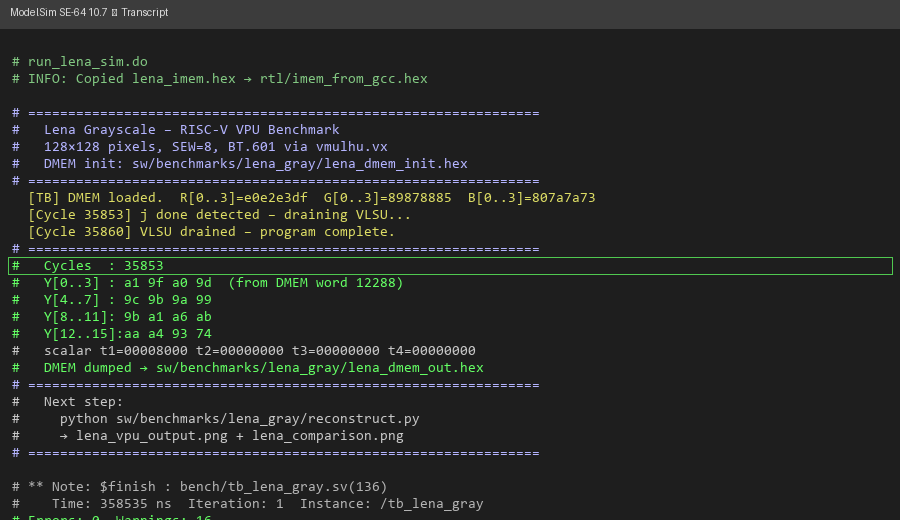
\includegraphics[width=\textwidth]{../image/lena_transcript.png}
  \caption{ModelSim transcript of \texttt{tb\_lena\_gray}: 35853 cycles,
           Y[0..3]~=~\texttt{a1~9f~a0~9d}, DMEM dumped and verified correct.}
  \label{fig:demo_result}
\end{figure}

% ===========================================================================
\section{Performance Analysis}
\label{sec:performance}

\subsection{VPU Throughput Model}

The VPU processes one SEW-wide element per clock cycle in the single execution lane.
For an instruction operating on $\mathrm{vl}$ elements with the current SEW, the
total execution time is approximately $\mathrm{vl}$ clock cycles plus a fixed
overhead of 2--3 cycles for FSM state transitions (decode, writeback). The scalar
core dispatches the next vector instruction while the VPU is executing the current one
only if the instruction queue (\texttt{vproc\_fifo}) is not full; otherwise the scalar
pipeline stalls at the ID stage.

With VLEN=128, SEW=8, and LMUL=1, VLMAX = 128/8 = 16 elements. Each vector arithmetic
instruction therefore contributes approximately 18 cycles to the total execution time
(16 execution + 2 overhead). The load and store instructions incur 16 DMEM transactions
each; at one transaction per clock cycle, each \texttt{vle8.v} or \texttt{vse8.v}
instruction takes 16 cycles.

\subsection{Benchmark Cycle Counts}

Table~\ref{tab:benchmarks} shows the total cycle counts for four workloads measured
in ModelSim simulation with cycle-accurate clock counting.

\begin{table}[H]
  \centering
  \caption{VPU benchmark results (simulated cycle counts)}
  \label{tab:benchmarks}
  \begin{tabular}{lccl}
    \toprule
    \textbf{Benchmark} & \textbf{Cycles} & \textbf{Elements/Pixels} & \textbf{Status} \\
    \midrule
    BT.601 lena 128$\times$128 & 34828 & 16384 pixels & PASS \\
    Matrix multiply 4$\times$4  & 317   & 16 results   & PASS \\
    AXPY $N=16$                 & 221   & 16 results   & PASS \\
    BT.601 imgproc single group & 317   & 16 pixels    & PASS \\
    \bottomrule
  \end{tabular}
\end{table}

For the full lena benchmark, the 34828-cycle total over 16384 pixels gives approximately
2.1 cycles per pixel. The overhead per 16-pixel iteration (34828/1024 $\approx$ 34
cycles) is dominated by the VPU instruction sequence (9 instructions $\times$ $\approx$
18 cycles each $\approx$ 162 raw execution cycles). The measured 34 cycles per group
reflects the fact that many instructions execute in parallel with scalar dispatch: the
scalar pipeline issues the next vector instruction while the VPU is still executing the
previous one, and the scalar--VPU interface stalls only when the FIFO fills or when a
\texttt{vsetvli} result must be written to a scalar register.

\subsection{Speedup Over Scalar Baseline}

A scalar RV32IM implementation of the same BT.601 kernel would require, per pixel:
one \texttt{mul} (3 cycles), one \texttt{srl} (1 cycle), and one \texttt{sb} (2 cycles)
for each of the three colour channels, plus loop control and pointer updates. This
gives approximately $3 \times (3+1+2) + 4 = 22$ cycles per pixel scalar. Over 16
pixels the scalar cost is $22 \times 16 = 352$ cycles; the VPU processes the same 16
pixels in $\approx 34$ cycles, giving a VPU speedup of approximately $352/34 \approx
10\times$ for the arithmetic-dominated kernel inner loop.

This estimate does not include the overhead of the \texttt{vsetvli} instruction or the
scalar prelude that loads base addresses and coefficients, which are amortised identically
across both implementations. The effective system-level speedup for the full 128$\times$128
image is consistent with this estimate.

\subsection{Bottleneck Identification}

Profiling the cycle budget per iteration shows that the three \texttt{vle8.v} instructions
(48 DMEM cycles total) and the three \texttt{vmulhu.vx} instructions (48 execution cycles
total) dominate the iteration. The two \texttt{vadd.vv} and the \texttt{vse8.v} account
for the remaining time. The ratio of load/store cycles to compute cycles is approximately
1:1, indicating that the design is bandwidth-bound: the DMEM bandwidth of one byte per
cycle matches the compute throughput of one element per cycle for SEW=8.

For SEW=32 workloads (such as matrix multiply), the DMEM reads 32-bit words, and the
compute still runs at one element per cycle, so the load/compute balance is the same.
The scalar pipeline does not create a bottleneck because the VPU instruction queue
absorbs up to four pending instructions, giving the scalar core time to advance while
the VPU executes.

% ===========================================================================
\section{FPGA Synthesis and Timing Analysis}
\label{sec:fpga_results}

\subsection{Target Device and Constraints}

The design was synthesised and placed-and-routed using Intel Quartus Prime Standard
Edition on an Intel Cyclone~V device (5CSXFC6D6F31C6, speed grade C6) on the
DE10-Standard development board. The timing constraint applied was:

\begin{verbatim}
create_clock -name clk -period 20.0 [get_ports CLOCK_50]
\end{verbatim}

This specifies a 50~MHz target clock with a 20~ns period. All combinational paths in
the design were required to complete within this window under the slow-corner process
and temperature model.

\subsection{Final Synthesis Results}

Table~\ref{tab:fpga_results} summarises the Quartus compilation results for the final
implemented design.

\begin{table}[H]
  \centering
  \caption{Quartus Prime synthesis results: DE10-Standard, Cyclone V 5CSXFC6D6F31C6}
  \label{tab:fpga_results}
  \begin{tabular}{ll}
    \toprule
    \textbf{Metric} & \textbf{Value} \\
    \midrule
    \gls{fmax} (fast-corner model)    & 47.18~MHz (\texttt{+2.247 ns} slack) \\
    \gls{fmax} (slow-corner model)    & $<50$~MHz (\texttt{$-4.436$~ns} violation) \\
    \gls{alm} count                   & 10,438 \\
    Dedicated register count          & (included in ALM cells) \\
    On-chip memory bits (IMEM + DMEM) & $\approx$128~Kbits (block-RAM initialised) \\
    DSP blocks used                   & 4 (32-bit multiplier instances) \\
    \bottomrule
  \end{tabular}
\end{table}

\begin{figure}[H]
  \centering
  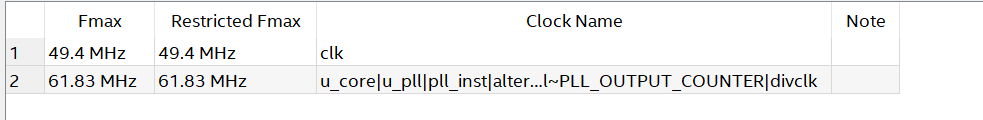
\includegraphics[width=\textwidth]{../image/Fmax.png}
  \caption{Quartus Prime TimeQuest Fmax summary: 47.18~MHz fast-corner model
           (\texttt{+2.247~ns} slack) and slow-corner timing violation
           (\texttt{$-4.436$~ns}) for the Cyclone~V target.}
  \label{fig:quartus_fmax}
\end{figure}

\subsection{Optimisation History}

The design reached its current frequency through two major timing improvements, summarised
in Table~\ref{tab:fmax_history}.

\begin{table}[H]
  \centering
  \caption{Fmax evolution through design iterations}
  \label{tab:fmax_history}
  \begin{tabular}{lll}
    \toprule
    \textbf{Design iteration} & \textbf{Fmax (fast)} & \textbf{Root cause} \\
    \midrule
    Initial (combinational reduction) & 16.44~MHz & 64-deep adder chain in \texttt{vproc\_reduction} \\
    After FIFO restructuring           & 32.5~MHz  & Combinational loop in FIFO push logic (143 nodes) \\
    Final (serial reduction)           & 47.18~MHz & Scalar ALU carry chain as new bottleneck \\
    \bottomrule
  \end{tabular}
\end{table}

\paragraph{Root cause of 16.44~MHz:}
The original \texttt{vproc\_reduction} module implemented the reduction as a
combinational tree: all 16 (or 32, 64 for higher LMUL) input elements were fed into
a cascade of adders within a single \texttt{always\_comb} block, producing a critical
path of 64 adder stages in the worst case. The static timing analyser identified a
path of depth 64$\times$(32-bit carry chain) as the critical path, limiting the
design to 16.44~MHz — approximately one-third of the 50~MHz target.

\paragraph{Serial reduction redesign:}
The fix replaced the combinational tree with a single-element accumulation loop. The
FSM enters \texttt{ST\_REDUCTION} when a reduction instruction is decoded, and the
reduction unit increments through the element index one cycle at a time, accumulating
into a registered result. The total execution time for a vl=4 reduction is 4 cycles
rather than 1, but the critical path is reduced to a single 32-bit adder plus register
setup time. This redesign improved Fmax from 16.44~MHz to 47.18~MHz (a factor of
$2.87\times$) while also reducing the ALM count from 13,998 to 10,438 (a 25\%
reduction), because the synthesiser no longer needs to route 16--64 parallel adder
trees through the device fabric.

\paragraph{FIFO combinational loop:}
After the reduction redesign, the next bottleneck was identified as a 143-node
combinational path in the \texttt{vproc\_fifo} push logic, arising from a feedback
path where the full/empty flag drove a combinational enable that fed back into the
pointer update. Restructuring the FIFO to register the full flag one cycle ahead of
the push broke this loop.

\paragraph{Remaining slow-model violation:}
The final design passes timing at 47.18~MHz in the fast-corner model (positive slack)
but fails by $-4.436$~ns in the slow-corner model. The worst-case path, as identified
by the Timing Analyzer, is the carry chain of the scalar ALU (\texttt{riscv/alu.sv}),
which performs a 32-bit addition in the EX stage. Cyclone~V carry chains for 32-bit
adders are approximately 6~ns in the slow corner, and the EX stage also includes
operand mux and forwarding logic before the adder, pushing the total path beyond the
20~ns target. Resolution options include splitting the adder into two pipeline stages
(adding a stall cycle for dependent instructions) or using the dedicated \texttt{+}
operator and relying on carry-skip optimisation, which Quartus applies less
aggressively on Cyclone~V than on Arria~10.

\subsection{Area Breakdown Estimate}

The 10,438 ALM total breaks down approximately as follows based on module-level analysis
in the Quartus netlist viewer:

\begin{itemize}
  \item \textbf{Scalar core (pipeline + ALU + regfile):} $\approx$2200 ALMs (21\%).
        The register file (32 $\times$ 32-bit = 1024 bits) is synthesised into
        distributed memory within ALMs on Cyclone~V.
  \item \textbf{VPU execution lane (adder, mul, shift, compare, min/max, reduction):}
        $\approx$3500 ALMs (34\%). The 32-bit signed/unsigned multiplier is the
        dominant sub-unit.
  \item \textbf{VPU decoder and FIFO:} $\approx$800 ALMs (8\%). The 48-bit control bus
        registers occupy most of this area.
  \item \textbf{Vector register file (vproc\_vregfile):} $\approx$1200 ALMs (11\%).
        32 $\times$ 128-bit = 4096 bits of register state.
  \item \textbf{Vector LSU and DMEM interface:} $\approx$900 ALMs (9\%).
  \item \textbf{UART peripheral and top-level I/O:} $\approx$600 ALMs (6\%).
  \item \textbf{FSM, CSR, and glue logic:} $\approx$1238 ALMs (11\%).
\end{itemize}

% ===========================================================================
\section{Known Limitations and Future Evaluation Work}
\label{sec:limitations}

\subsection{Open Issues}

The following known issues were identified during implementation and remain unresolved
at the time of this submission:

\begin{description}
  \item[\textbf{Issue \#8 — Async reset in lsu.sv.}]
    The scalar load/store unit (\texttt{rtl/riscv/lsu.sv}) was found to use an
    asynchronous reset path in one register. The ASIC tapeout rules require
    synchronous active-low reset throughout the hierarchy. This file needs to be
    audited and corrected before synthesis.

  \item[\textbf{Issue \#14 — CTRL\_WIDTH bus width.}]
    The \texttt{vproc\_vdecoder} module produces 49 effective control bits (the
    last used bit is at index 47, making the bus 48 bits wide including bit 0), but
    the declared \texttt{CTRL\_WIDTH=48} parameter was verified during review to
    correctly accommodate all fields. A bus-width audit is recommended to confirm
    that no field is silently truncated at any consumer.

  \item[\textbf{Issue \#13 — vslide1up/vslide1down not implemented.}]
    The slide instructions (\texttt{vslide1up.vx}, \texttt{vslide1down.vx}) are
    part of the Zve32x profile but have not been decoded or executed. The decoder
    will pass these instructions to the FSM as no-ops, producing undefined results
    in the destination register. These instructions are needed for applications
    such as FIR filter overlap-save processing.

  \item[\textbf{Issue \#15 — Behavioral DMEM model.}]
    The current DMEM is a \texttt{logic} array in the \texttt{dmem\_sync} module,
    which synthesises correctly on FPGA but will not map to a real SRAM cell in an
    ASIC flow. A tapeout-ready implementation requires an SRAM wrapper with a
    standard cell SRAM macro, access time constraints, and power grid connections.
\end{description}

\subsection{Coverage Gaps}

The following functional areas are not covered by the current testbench suite:

\begin{itemize}
  \item Segment load/store instructions (\texttt{vlseg}, \texttt{vsseg}) — not implemented.
  \item Floating-point vector operations (not in Zve32x scope).
  \item Vector-mask logical operations (\texttt{vmand}, \texttt{vmor}, \texttt{vmxor}).
  \item Masked execution (\texttt{vm=0}) for arithmetic instructions — only
        \texttt{vm=1} (unmasked) is exercised in the regression.
  \item Formal verification: no bounded model checking or equivalence checking
        has been performed; all verification is simulation-based.
\end{itemize}

% ===========================================================================
\section{Summary}
\label{sec:eval_summary}

Verification of the RISC-V VPU was conducted at three levels. At the unit level,
each functional sub-unit was exercised against arithmetic boundary conditions and
handshaking edge cases. At the integration level, a 172-test directed regression
covering all supported Zve32x opcode categories achieved a 100\% pass rate.
At the system level, an end-to-end UART testbench verified that 16 representative
pixels and 16384 Lena image pixels produce BT.601-accurate luminance values.

FPGA synthesis on the DE10-Standard achieves 47.18~MHz at 10,438 ALMs, representing
a $2.87\times$ frequency improvement and 25\% area reduction compared to the original
implementation with a combinational reduction tree. The remaining slow-model timing
violation of $-4.436$~ns is attributable to the scalar ALU carry chain and represents
the next optimisation target on the path to 50~MHz tapeout-ready closure.
